\section{Tổng quan bài toán}
Bài toán của báo cáo là phân loại hình 3D. Cụ thể hơn thì báo cáo sẽ làm việc về bài toán Point Cloud classification. Point Cloud Classification là một bài toán trong lĩnh vực Machine Learning và Computer Vision, đặc biệt liên quan đến việc xử lý dữ liệu 3D. Point Cloud là một tập hợp các điểm trong không gian ba chiều (3D), mỗi điểm được xác định bởi tọa độ (x, y, z) và đôi khi kèm theo các thông tin khác như màu sắc, cường độ ánh sáng, hay các đặc điểm khác. Các điểm này được thu thập từ các cảm biến 3D như LiDAR, máy quét 3D, hoặc từ các hình ảnh 2D thông qua các kỹ thuật như Structure from Motion (SfM).

Mục tiêu của bài toán Point Cloud Classification là phân loại toàn bộ đám mây điểm thành các nhãn (labels) khác nhau, chẳng hạn như xác định một đám mây điểm thuộc về một loại đối tượng nào đó (ví dụ: ô tô, người, cây cối, tòa nhà).

\begin{figure}[H]
    \centering
    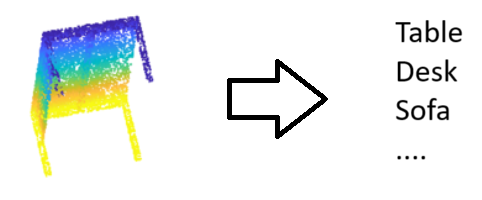
\includegraphics[width=0.7\linewidth]{Images/tong_quan_bt.png}
\end{figure}

Một số thách thức chính trong Point Cloud Classification bao gồm:
\begin{itemize}
    \item Không gian đầu vào có kích thước lớn: Đám mây điểm thường chứa hàng nghìn đến hàng triệu điểm, gây khó khăn cho việc xử lý và tính toán.

    \item Thiếu thông tin cấu trúc: Khác với hình ảnh 2D có cấu trúc lưới cố định, các điểm trong point cloud không có thứ tự cố định và không có cấu trúc mạng lưới rõ ràng, làm cho việc áp dụng các phương pháp truyền thống như Convolutional Neural Networks (CNN) trở nên khó khăn.

    \item Tính không đồng nhất: Point cloud có thể có mật độ không đồng nhất, nghĩa là một số vùng có thể chứa nhiều điểm hơn các vùng khác, tạo ra sự bất đối xứng trong dữ liệu.

\end{itemize}

\section{Dữ liệu sử dụng}
Ở đây, báo cáo sẽ sử dụng bộ dữ liệu về Point Cloud là bộ dữ liệu ModelNet10\cite{data_modelnet10}. ModelNet10 là một bộ dữ liệu chuẩn trong lĩnh vực xử lý dữ liệu 3D, được sử dụng phổ biến trong các nghiên cứu và thí nghiệm liên quan đến Point Cloud Classification và 3D Object Recognition. Bộ dữ liệu này được giới thiệu lần đầu tiên bởi các nhà nghiên cứu tại Princeton University trong bài báo "3D ShapeNets: A Deep Representation for Volumetric Shapes"\cite{data_modelnet10} vào năm 2015.

\begin{figure}[H]
    \centering
    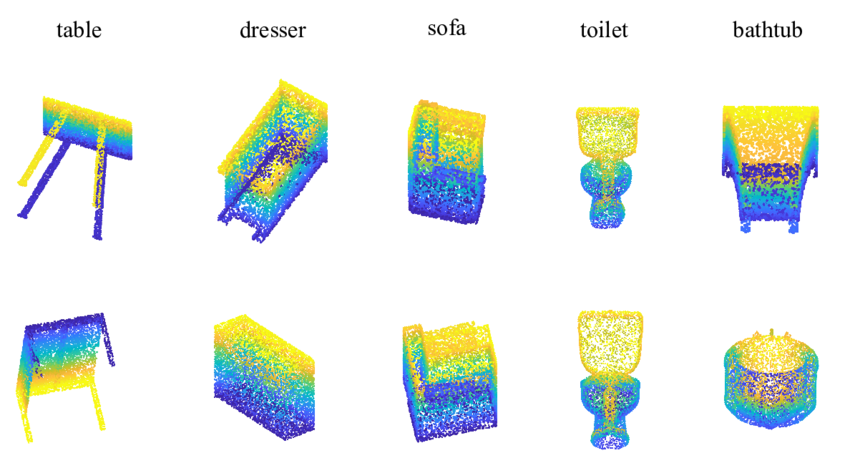
\includegraphics[width=0.8\linewidth]{Images/TFN/data_img.png}
    \caption{Ảnh minh họa một số dữ liệu trong tập dữ liệu ModelNet10}
\end{figure}

ModelNet10 bao gồm khoảng \textbf{3991} dữ liệu 3D được trích xuất từ các đối tượng trong thế giới thực và được sắp xếp thành 10 danh mục khác nhau. Những danh mục này bao gồm: Bed (Giường), Chair (Ghế), Desk (Bàn làm việc), Dresser (Tủ ngăn kéo), Monitor (Màn hình), Nightstand (Tủ đầu giường), Sofa (Ghế sofa), Table (Bàn), Toilet (Bồn cầu), Bathtub (Bồn tắm)

\section{Phương pháp thực nghiệm}
Ở đây, báo cáo sẽ chỉ thực nghiệm để thấy được sự hữu ích của các mạng \textit{equivariant deep learning} trong bài toán liên quan đến dữ liệu 3D. Cụ thể hơn, báo cáo chỉ sử dụng TFN để cho thấy rằng dữ liệu được training là dữ liệu chưa xoay đi một góc nào đấy. Do đó, sau khi training xong, báo cáo sẽ xay dữ liệu một cách ngẫu nhiên rồi sau đó cho mô hình dự đoán.

Về phần dữ liệu, do hạn chế về mặt phần cứng là 15GB VRAM của Google Colab, báo cáo không thể training hết được toàn bộ dữ liệu do có một số dữ liệu có rất nhiều điểm (khoảng hơn 1000 điểm). Do đó, với mỗi loại nhãn của dữ liệu, báo cáo sẽ lấy một điểm dữ liệu cho mỗi loại nhãn rồi sau đó training mô hình TFN với dữ liệu này.

Về phần mô hình, báo cáo sử dụng thư viện E3NN để xây dựng mô hình TFN. TFN sẽ có hai layer do số lượng dữ liệu ít (10 dữ liệu). Giữa hai layer này sẽ có một hàm kích hoạt của thư viện E3NN có tên là Gate. Kích thước đầu ra cuối cùng sẽ là 10 với hàm kích hoạt là Softmax tượng trưng cho xác suất mà một dữ liệu thuộc vào từng class. 

Mô hình sẽ được huấn luyện với 200 epochs với kích thước batch là 10. Hàm mất mát được sử dụng là Cross-Entropy loss và thuật toán tối ưu là Adam với learning rate là $10^{-3}$.

\begin{table}[h!]
\centering
 \begin{tabular}{|c | c |} 
 \hline
    Thiết bị huấn luyện & T4 GPU (Google Colab)\\
 \hline
    Số epochs & 200\\
 \hline
    Kích thước batch & 10\\
 \hline
    Hàm mất mát & Cross - Entropy\\
 \hline
    Thuật toán tối ưu & Adam\\
 \hline
    Hệ số học & $10^{-3}$\\
 \hline
 \end{tabular}
 \caption{Bảng thống kê các thông số huấn luyện mô hình}
\end{table}

\section{Kết quả thực nghiệm và đánh giá}
Sau quá trình training, mô hình đạt được độ chính xác là 80\% . Điều này cho thấy rằng mô hình vẫn chưa phân loại tốt hoàn toàn vì một phần là thiếu dữ liệu hoặc có thể là do có một số dữ liệu có cấu trúc khá là tương đồng nên mô hình chưa thể nhận biết được. Hình \ref{fig:acc_track} dưới đây là biểu đồ theo dõi chất lượng dự đoán của mô hình.

\begin{figure}[H]
    \centering
    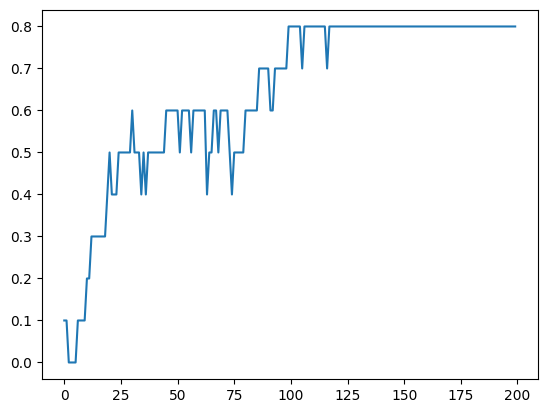
\includegraphics[width=0.7\linewidth]{Images/TFN/acc_re.png}
    \caption{Biểu đồ theo dõi tính độ chính xác của mô hình trong quá trình training}
    \label{fig:acc_track}
\end{figure}

Từ biểu đồ có thể thấy độ chính xác ban đầu khá thấp nhưng tăng dần qua các epoch, cho thấy mô hình đang học và cải thiện dần. Tuy nhiên, trong quá trình training, độ chính xác dao động khá nhiều, đặc biệt là ở giai đoạn giữa, điều này có thể chỉ ra rằng mô hình phải tinh chỉnh khá nhiều để khớp với dữ liệu hơn. Cuối quá trình training, độ chính xác dần ổn định và đạt mức khoảng 0.8, nghĩa là mô hình có khả năng dự đoán đúng khoảng 80\% dữ liệu.

Để thấy được độ hiệu quả của mô hình khi dự đoán dữ liệu đối với tác động của phép xoay, báo cáo sẽ xoay từng dữ liệu một góc bất kỳ trong không gian 3 chiều rồi cho mô hình dự đoán. Hình \ref{fig:equi_re} cho thấy cái nhìn tổng quan về hiệu suất của mô hình với các hình có tiêu đề chỉ có chữ label là dữ liệu gốc còn đối với dữ liệu còn lại là dữ liệu đã được xoay.

\begin{figure}[H]
    \centering
    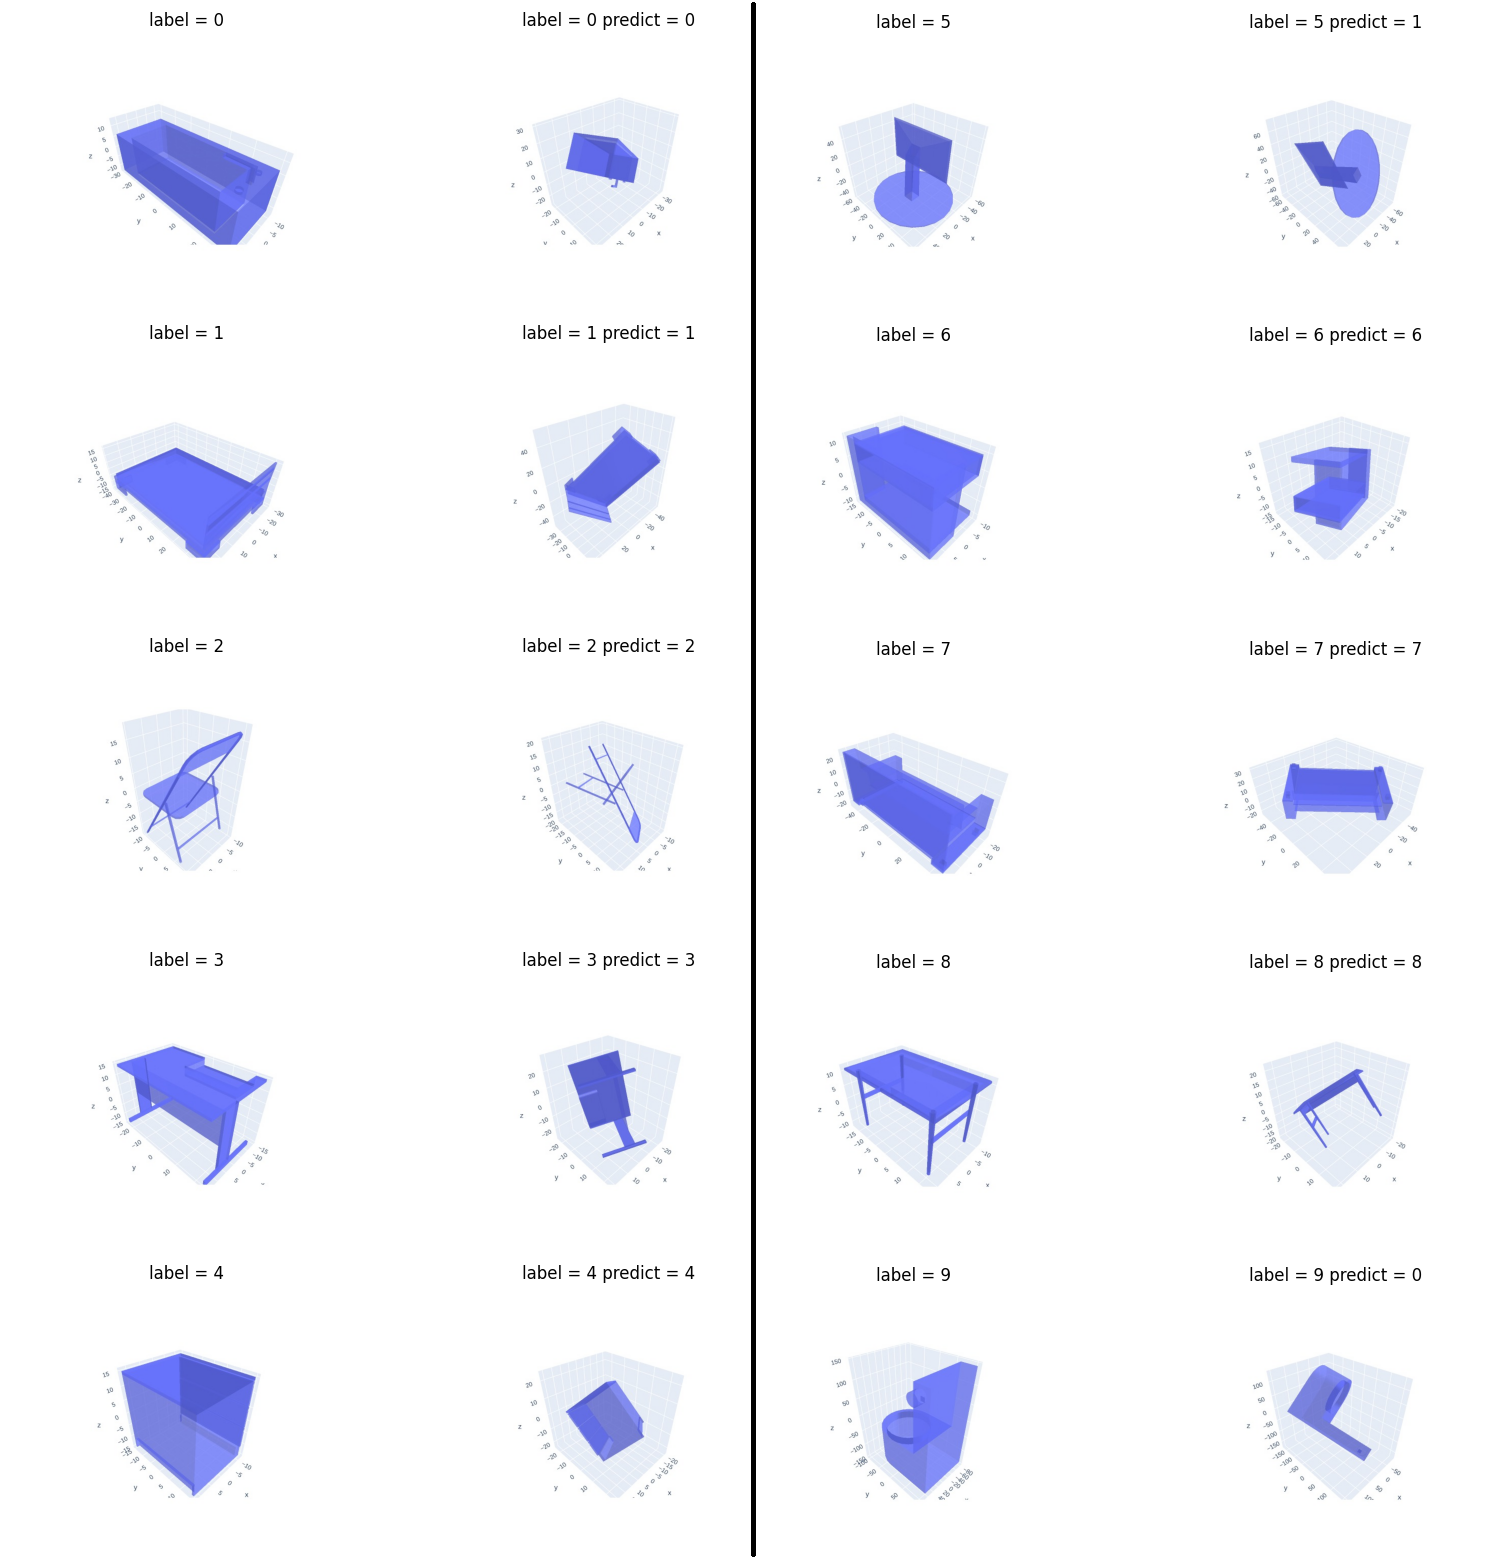
\includegraphics[width=1\linewidth]{Images/TFN/result.png}
    \caption{Hình ảnh thống kê kết quả dự đoán của mô hình}
    \label{fig:equi_re}
\end{figure}

Có thể thấy mô hình hoạt động khá tốt khi dự đoán chính xác 8/10 dữ liệu. Đối với những dữ liệu dự đoán sai thì chúng ta sẽ cần phải thêm dữ liệu đối với mô hình hoặc là thay đổi cấu trúc của mô hình để đạt được hiệu quả cao hơn.